%%==================================================
%% chapter01.tex for SJTU Master Thesis
%% based on CASthesis
%% modified by wei.jianwen@gmail.com
%% version: 0.3a
%% Encoding: UTF-8
%% last update: Dec 5th, 2010
%%==================================================

%\bibliographystyle{sjtu2} %[此处用于每章都生产参考文献]
\chapter{背景介绍}
\label{chap:background}

无线网络中的一个基本问题是如何在系统可靠性与网络传输性能之间进行有效平衡,对于高速移动网络而言,首先要保证其系统可靠性以实现信息的可靠传输;而无线局域网络则更关注网络的传输性能,包括网络吞吐量及覆盖范围等。信道状态和链路质量作为无线网络可靠性与传输性能的衡量指标,同时也是网络运行与优化的重要参数,因此两者的准确高效的测量对于移动网络可靠性与传输性能的有效平衡至关重要。本文主要针对高速移动网络和无线局域网络中的信道估计与链路测试问题,对移动网络的通信质量测试进行详细分析,并通过算法设计、系统实现与实验测试对移动网络通信质量测试算法进行评估。

\section{移动无线网络}
\label{sec:mobile}


\subsection{高速移动网络}
\label{sec:gsmr}

在高速铁路的快速发展的过程中,列车的安全稳定运行至关重要,要实现高铁的安全稳定高速运行,必须实时地对整个高铁系统进行安全监测。其中列控系统保证高铁系统的可靠运行,GSM-R无线网络则是列控系统中的关键环节,同时又是系统中最脆弱的部分。GSM-R网络是专门应用于铁路环境中的综合数字调度移动通信网络,如图 \ref{fig:gsmrservice} 所示,GSM-R网络承载了高速铁路的列车运行状态数据传输、列车控制数据传输、区间移动公务通信、应急指挥通信等业务,因此对GSM-R网络进行实时监测具有重要意义。

\begin{figure}[!htp]
\centering
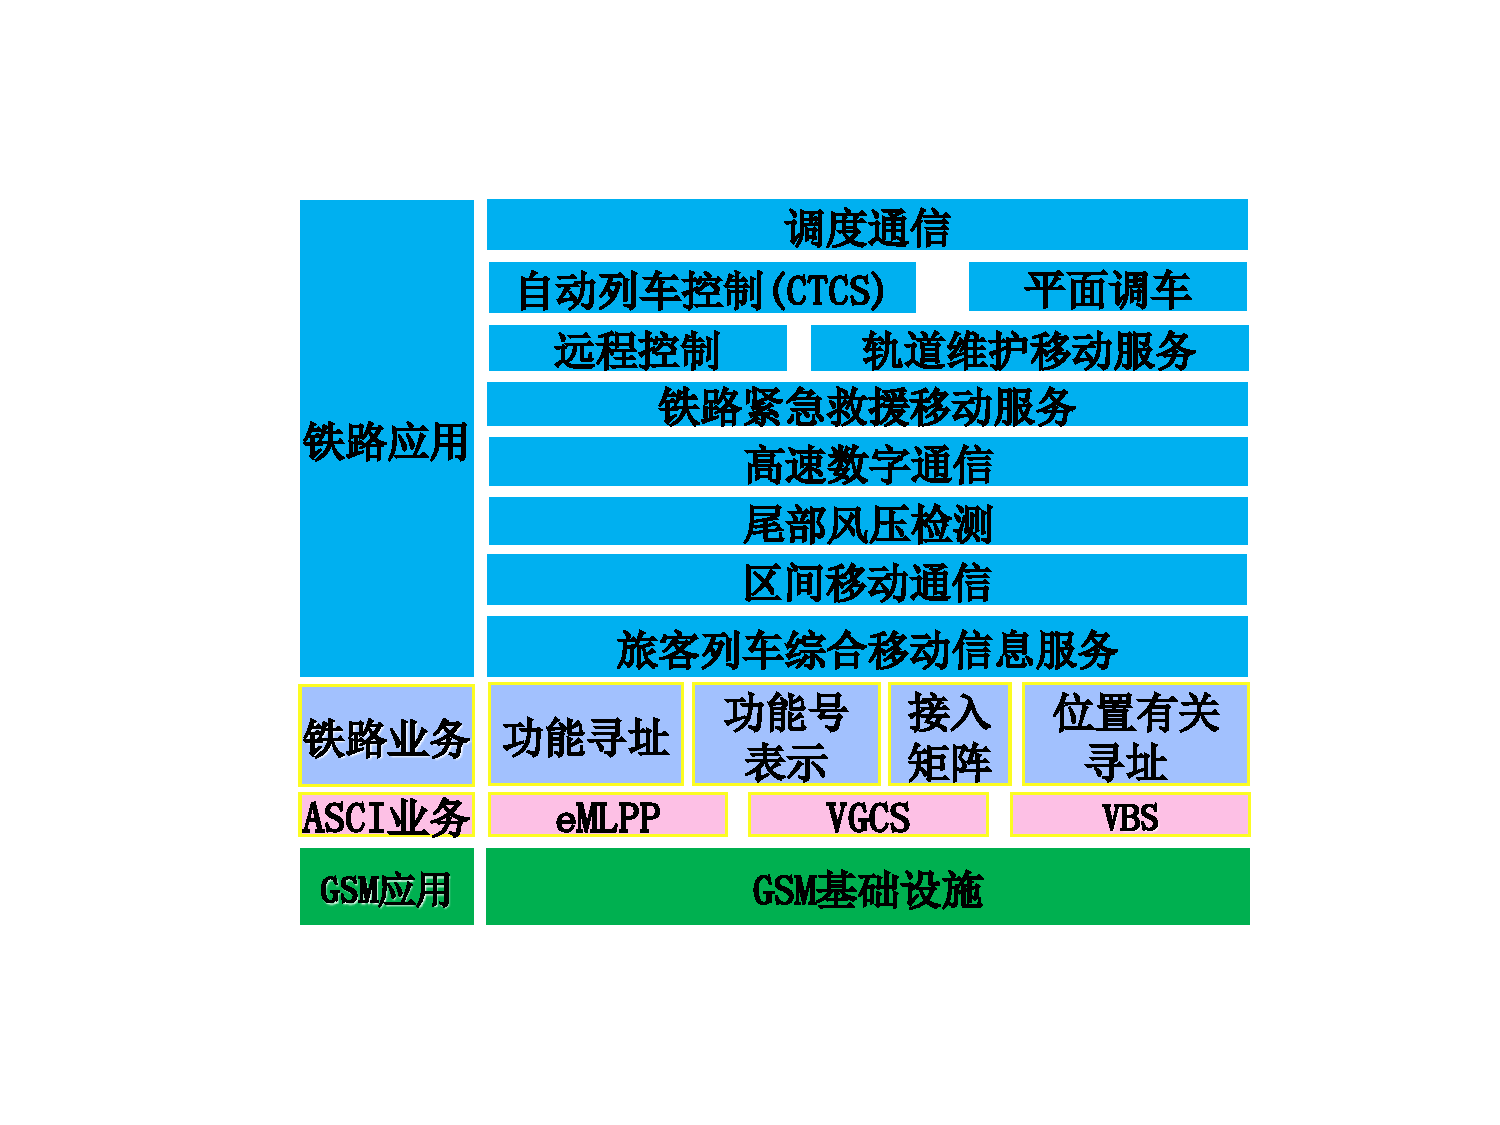
\includegraphics[width=0.6\textwidth]{chap1/gsmrservice.pdf}
\bicaption[fig:gsmrservice]{GSM-R网络业务模型}{GSM-R网络业务模型}{Fig}{Service model of GSM-R networks}
\end{figure}

目前我国的GSM-R数字移动通信系统由七个子系统构成:网络交换子系统(SSS)、基站子系统(BSS)、操作维护子系统(OSS)、通用分组无线业务子系统(GPRS)、智能网子系统(IN)、固定接入交换子系统(FAS)和终端子系统,如图 \ref{fig:gsmr} 所示。GSM-R系统的各个功能单元通过不同的接口进行连接,使各组成单元在物理上和逻辑上遵守特定的协议。GSM-R系统测试的主要应用到的接口有空中接口、Abis接口、A接口、PRI接口等,其中空中接口是移动台与基站之间的通信接口,用于移动台与GSM-R系统固定部分之间的通信,其物理连接通过无线链路实现,它的特点是完全标准化。

在GSM-R网络的通信过程中,大部分的信令都是和移动台相关,从图 \ref{fig:gsmr} 中可以看出,虽然移动台只和基站之间存在接口,但发往基站和从基站发往移动台的信令消息中还包括了移动台与GSM-R网络中其他设备之间的通信信息,即要在无线接口上传输各种不同的协议。同时,由于空中接口为无线链接,其可靠性是GSM-R网络能够正常运行的基础,因此对GSM-R的空中接口进行实时监测有着非常重要的意义。

\begin{figure}[!htp]
\centering
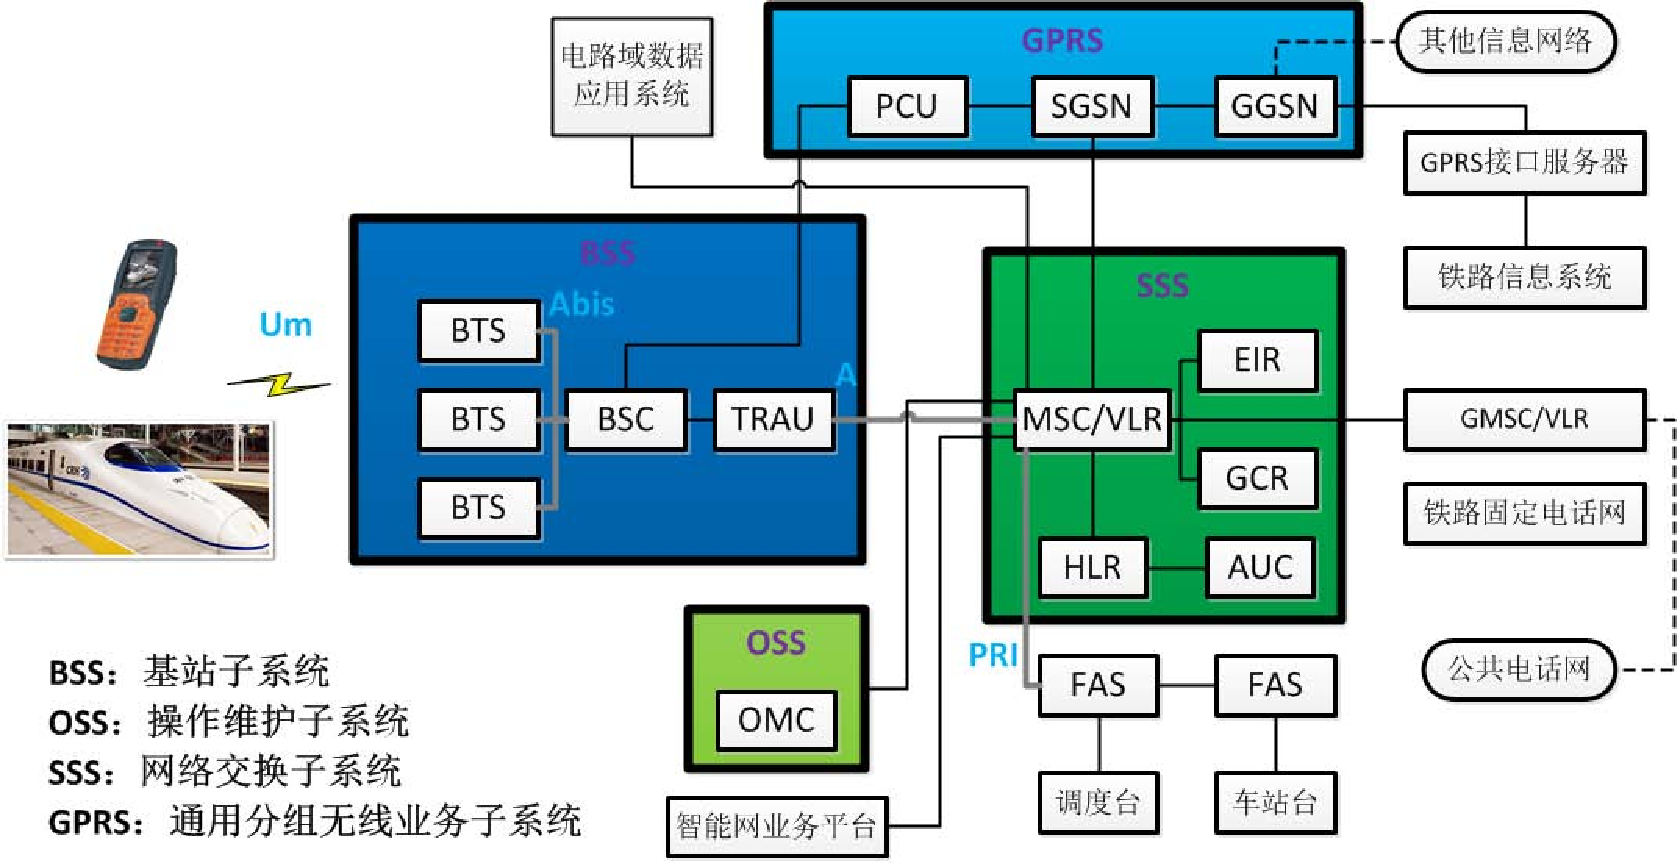
\includegraphics[width=0.9\textwidth]{chap1/gsmr.pdf}
\bicaption[fig:gsmr]{GSM-R网络基本结构}{GSM-R网络基本结构}{Fig}{Architecture of GSM-R networks}
\end{figure}

\subsection{无线局域网络}
\label{sec:80211n}

无线局域网络经历了快速的发展,

802.11n网络由于采用了MIMO-OFDM技术,显著提升了无线局域网络的传输性能与覆盖范围,

\begin{table}[!htp]
\renewcommand{\arraystretch}{1}
\bicaption[tab:feature]{802.11网络基本参数}{802.11网络基本参数}{Table}{Features and settings of 802.11 networks}
\centering
\begin{threeparttable}[b]
\begin{tabular}{ccccc}
\hline
         & 802.11a  & 802.11b    & 802.11g       & 802.11n \\
\hline
调制方式 & OFDM     & DSSS/CCK   & OFDM DSSS/CCK & SDM/OFDM \\
%\cline{2}
频率     & 5GHz     & 2.4GHz     & 2.4GHz        & 2.4/5GHz \\
%\cline{2}
信道带宽 & 20MHz    & 25MHz      & 25MHz         & 20/40MHz \\
%\cline{2}
传输速率 & 6-54Mbps & 5.5/11Mbps & 1-54Mbps     & 6-600Mbps \\
\hline
\end{tabular}
\end{threeparttable}
\end{table}

物理层技术主要包括多天线技术、正交频分复用技术以及信道绑定技术等,

\begin{figure}[!htp]
\centering
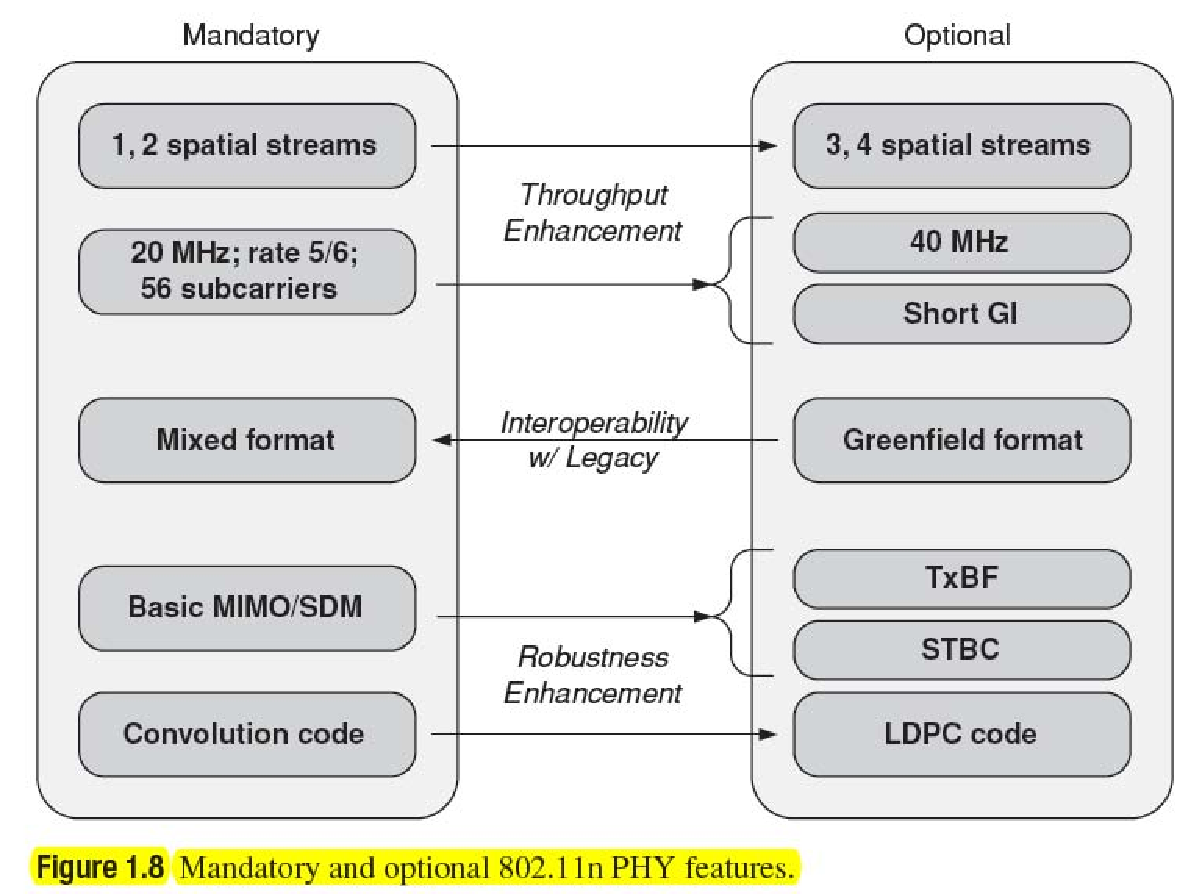
\includegraphics[width=0.5\textwidth]{chap1/PHYfeather.pdf}
\bicaption[fig:phyfeather]{802.11n网络PHY特性}{802.11n网络PHY特性}{Fig}{Feather of 802.11n Networks}
\end{figure}

\subsubsection{物理层}
\begin{itemize}
  \item Spatial Diversity
  \item Channel Bonding
\end{itemize}

链路层技术主要包括短保护间隔、帧聚合技术以及块应答机制等

\begin{figure}[!htp]
\centering
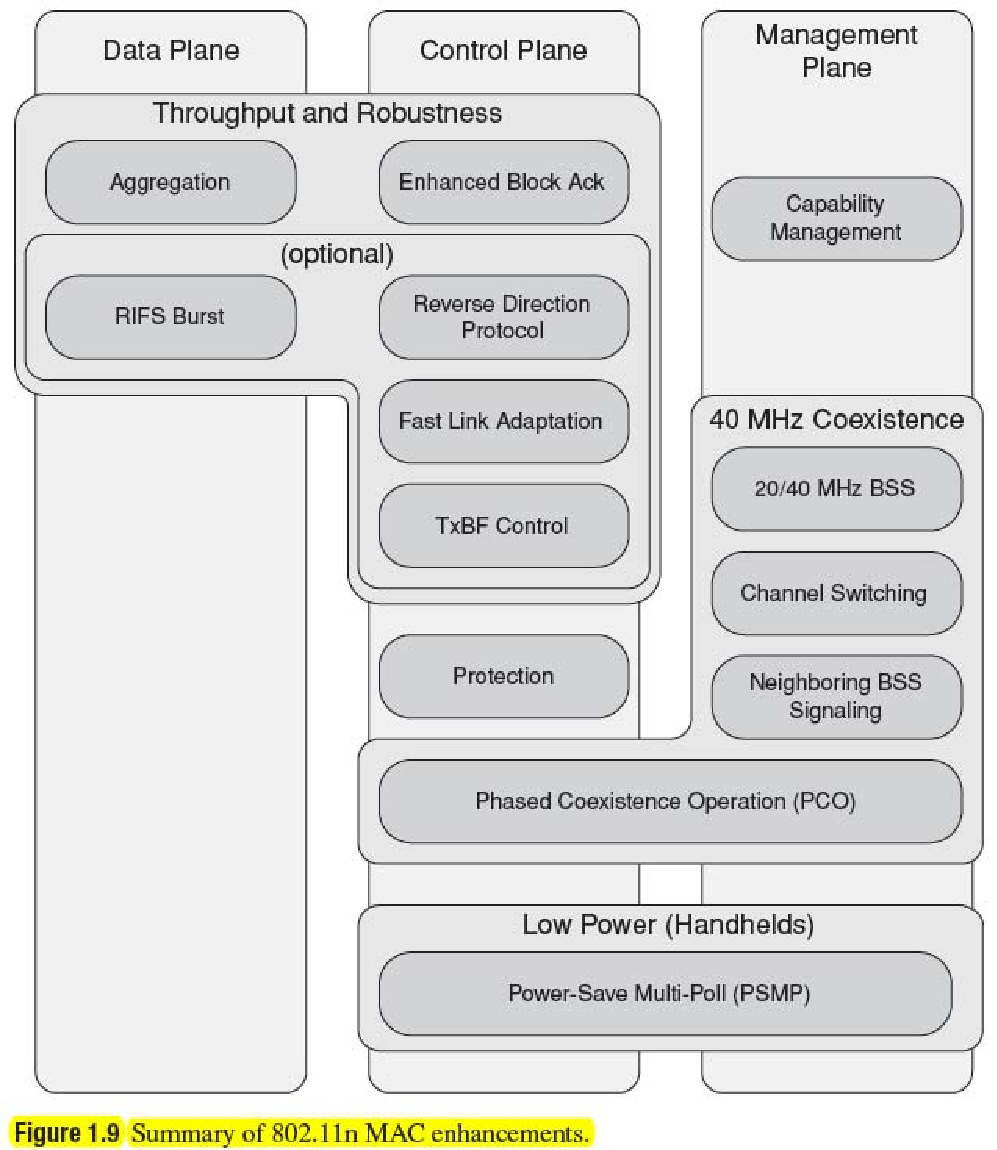
\includegraphics[width=0.5\textwidth]{chap1/MACfeather.pdf}
\bicaption[fig:macfeather]{802.11n网络MAC特性}{802.11n网络MAC特性}{Fig}{Feather of 802.11n Networks}
\end{figure}

\subsubsection{链路层}
\begin{itemize}
  \item Frame Aggregation
  \item Streamlined ACK
\end{itemize}

%\begin{table}[!htp]
%\renewcommand{\arraystretch}{1}
%\bicaption[tab:mcs]{802.11n网络MCS索引}{802.11n网络MCS索引}{Table}{MCS index of 802.11n}
%\centering
%\begin{threeparttable}[b]
%\begin{tabular}{c|c|c|ccc}
%\hline
%  Channel & MCS & Rate(Mbps) & $\beta_-$ & $\beta_0$ & $\beta_+$ \\
%\hline
%  \multirow{8}{*}{HT20/LGI} & 0 &  6.5 & -70 & -65 & -60 \\
%\cline{2}
%                            & 1 & 13.0 & -70 & -65 & -60 \\
%\cline{2}
%                            & 2 & 13.0 & -70 & -65 & -60 \\
%\cline{2}
%                            & 3 & 13.0 & -70 & -65 & -60 \\
%\cline{2}
%                            & 4 & 13.0 & -70 & -65 & -60 \\
%\cline{2}
%                            & 5 & 13.0 & -70 & -65 & -60 \\
%\cline{2}
%                            & 6 & 13.0 & -70 & -65 & -60 \\
%\cline{2}
%                            & 7 & 13.0 & -70 & -65 & -60 \\
%\hline
%  \multirow{8}{*}{HT20/SGI} & 0 &  6.5 & -70 & -65 & -60 \\
%\cline{2}
%                            & 1 & 13.0 & -70 & -65 & -60 \\
%\cline{2}
%                            & 2 & 13.0 & -70 & -65 & -60 \\
%\cline{2}
%                            & 3 & 13.0 & -70 & -65 & -60 \\
%\cline{2}
%                            & 4 & 13.0 & -70 & -65 & -60 \\
%\cline{2}
%                            & 5 & 13.0 & -70 & -65 & -60 \\
%\cline{2}
%                            & 6 & 13.0 & -70 & -65 & -60 \\
%\cline{2}
%                            & 7 & 13.0 & -70 & -65 & -60 \\
%\hline
%\end{tabular}
%\end{threeparttable}
%\end{table}


\section{通信质量测试}
\label{sec:measure}

Calculate throughput based on the average A-MPDU length, taking into account the expected number of retransmissions and their expected length.

1. Packet Delivery Ratio: $1-\frac{Retries+Failed}{Transmitted}$

2. Frame Delivery Ratio: $1-\frac{A\text{-}MPDUs * Retries + Failed MPDUs}{A\text{-}MPDUs * Retries+1}$

3. Efficient Date Rate: $DateRate * PDR$

4. Efficient Throughput: $Throughput * PDR$

\subsection{物理层信道状态估计}
\label{sec:phy}


\subsection{链路层链路质量测试}
\label{sec:mac}

\begin{table}[!htp]
\renewcommand{\arraystretch}{1}
\bicaption[tab:mcs]{802.11n网络MCS索引}{802.11n网络MCS索引}{Table}{MCS index of 802.11n}
\centering
\begin{threeparttable}[b]
\begin{tabular}{cccccc}
\hline
  \multirow{2}{*}{MCS} & \multirow{2}{*}{Modulation} & \multirow{2}{*}{Code Rate} & \multirow{2}{*}{Rate (Mbps)} & \multicolumn{2}{c}{Sensitivity (dBm)} \\
\cline{5-6}
  & & & & Typical & Max \\
\hline
  0 & BPSK & 1/2 & 6.5 & -94 & -85 \\
%\cline{2}
  1 & QPSK & 1/2 & 13.0 & -92 & -82 \\
%\cline{2}
  2 & QPSK & 3/4 & 19.5 & -90 & -80 \\
%\cline{2}
  3 & 16 QAM & 1/2 & 26.0 & -87 & -77 \\
%\cline{2}
  4 & 16 QAM & 3/4 & 39.0 & -84 & -73 \\
%\cline{2}
  5 & 64 QAM & 2/3 & 52.0 & -79 & -69 \\
%\cline{2}
  6 & 64 QAM & 3/4 & 58.5 & -78 & -68 \\
%\cline{2}
  7 & 64 QAM & 5/6 & 65.0 & -76 & -67 \\
\hline
\end{tabular}
\end{threeparttable}
\end{table}

\subsubsection{速率控制}

  1. sample
    \begin{enumerate}
      \item The rate chosen by sample did not alter to match changes in the radio
	    environment.
      \item Higher throughput (between two nodes) could often be achieved by fixing
	    the bitrate of both nodes to some value.
      \item After a long period of operation, "sample" appeared to be stuck in a low
	    data rate, and would not move to a higher data rate.
    \end{enumerate}

  2. minstrel
    EWMA calculations are used to process the success history of each rate. On
	completion of the calculation, a decision is made as to the rate which has the
	best throughput, second best throughput, and highest probability of success.
	This data is used for populating the retry chain during the next 100 ms.

    The EWMA calculation is carried out 10 times a second, and is run for each
	rate. This calculation has a smoothing effect, so that new results have a
	reasonable (but not large) influence on the selected rate. However, with time,
	a series of new results in some particular direction will predominate.

    Minstrel spends a particular percentage of frames, doing "look
	around" i.e. randomly trying other rates, to gather statistics. The percentage
	of "look around" frames, is set at boot time via the module parameter
	"ath\_look-around\_rate" and defaults to $10\%$. The distribution of look-around
	frames is also randomized somewhat to avoid any potential "strobing" of
	look-around between similar nodes.

    The contention window size does vary with traffic class. For example, video	and voice have a contention window min of 3 and 2 microseconds respectively. Currently, minstrel does not check traffic class.	Calculating the throughput based on traffic class and bit rate and variable packet size will significantly complicate the code and require many more sample packets. More sample packets will lower the throughput achieved. Thus, our view is that for this release, we should take a simple (but reasonable) approach that works stably and gives good throughput.

  3. ath9k